\title{COMP3702 - Assignment 2}
\author{Roy Portas - 43560846}
\date{\today}

\documentclass[12pt]{article}
\usepackage{graphicx}
\usepackage{geometry}
\usepackage{listings}
\geometry{
    a4paper,
    margin=1in
}

\begin{document}
    \maketitle

    \section{Chosen Configuration Space}

    The chosen configuration space will be the area containing all valid chair movements. Below is an example of what the configuration space will look like.

    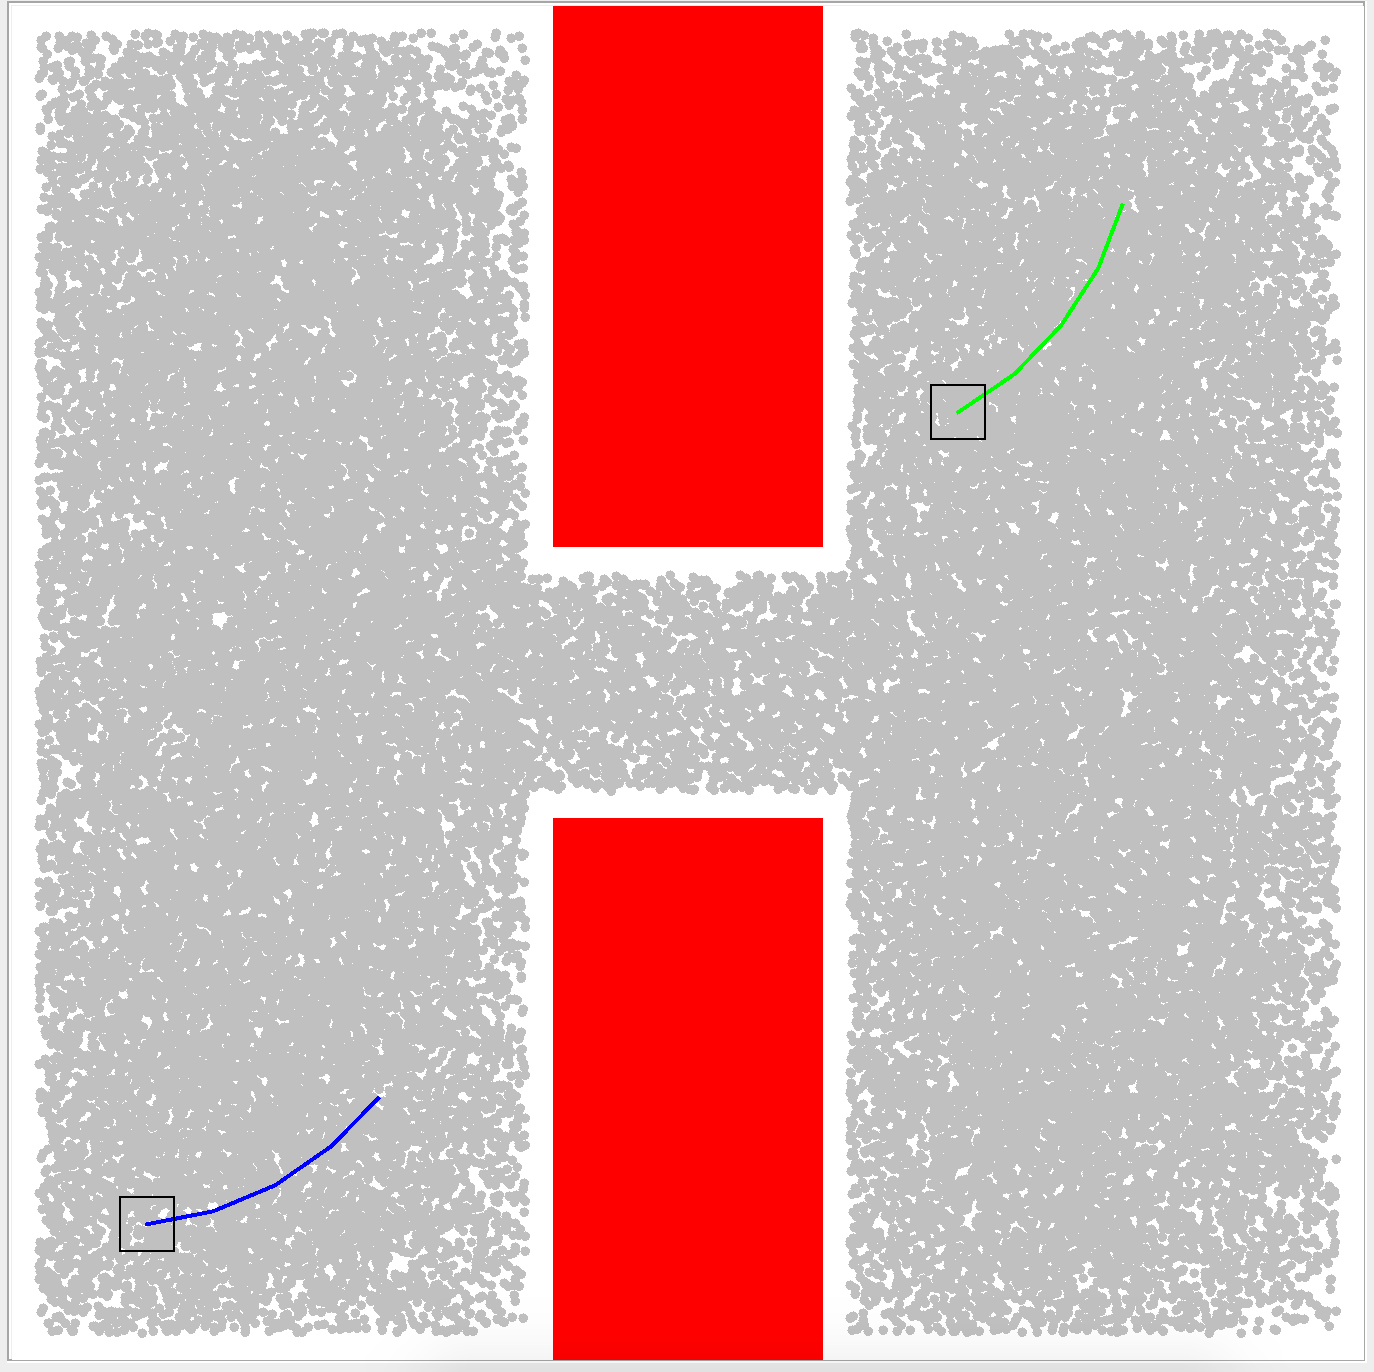
\includegraphics[scale=0.5]{resources/c-space.png}

    In the image above, the grey dots are the chair basepoints generated by the sampling strategy. It can be seen that the border of the grey area will be the configuration space, as the area outside of it is invalid for the chair to move.

    \section{Sampling Strategy}

    There are various sampling strategies that could work for the given problem, most notably:

    \begin{itemize}
        \item Sampling Near Obstacles
        
            This method is promising, since we are given all the obstacles at the start. Thus this sampling only needs to be done once. However since we are given the complete workspace, there are better choices for this problem.

        \item Sample Inside a Passage

            The obstacles for our problem can be sparse, with large distances between obstacles. Thus this strategy would not be an optimal choice.

        \item Using Workspace Information

            This strategy also looks promising, as we are given the complete workspace. Thus a possible solution is to sample the workspace randomly to create a discrete grid. The grid can then be converted into a search graph using rapidly exploring random trees. Additionally supporting code which does the workspace collision checking is provided, this will save development time and thus this strategy was chosen.
    \end{itemize}

    The workspace sampling strategy was chosen as the code is already provided and will suit the problem at hand/

    \subsection{Implementation}

    The strategy was implemented using the following pseudocode:

    \begin{lstlisting}
        N = Number of required samples
        samples = List of valid samples

        while samples.length < N:
            
            x = Random configuration in the workspace
            if x is a valid configuration:
                add x to samples

    \end{lstlisting}

    The end result of this will be a list of valid configurations in the workspace. This list is later used to create a KDTree for searching.

    \section{What will cause the program to succeed}

    In theory as long as there is a number of valid configurations between the start and destination, the program will succeed. However the chances are increased if the number of samples is larger.

    \section{What will cause the program to fail}

    The program will fail if the number of samples is insufficient.
\end{document}
